\section{Nestedness: From Ecology to Finance}

\begin{frame}
\frametitle{What is Nestedness?}

\begin{figure}
    \centering
    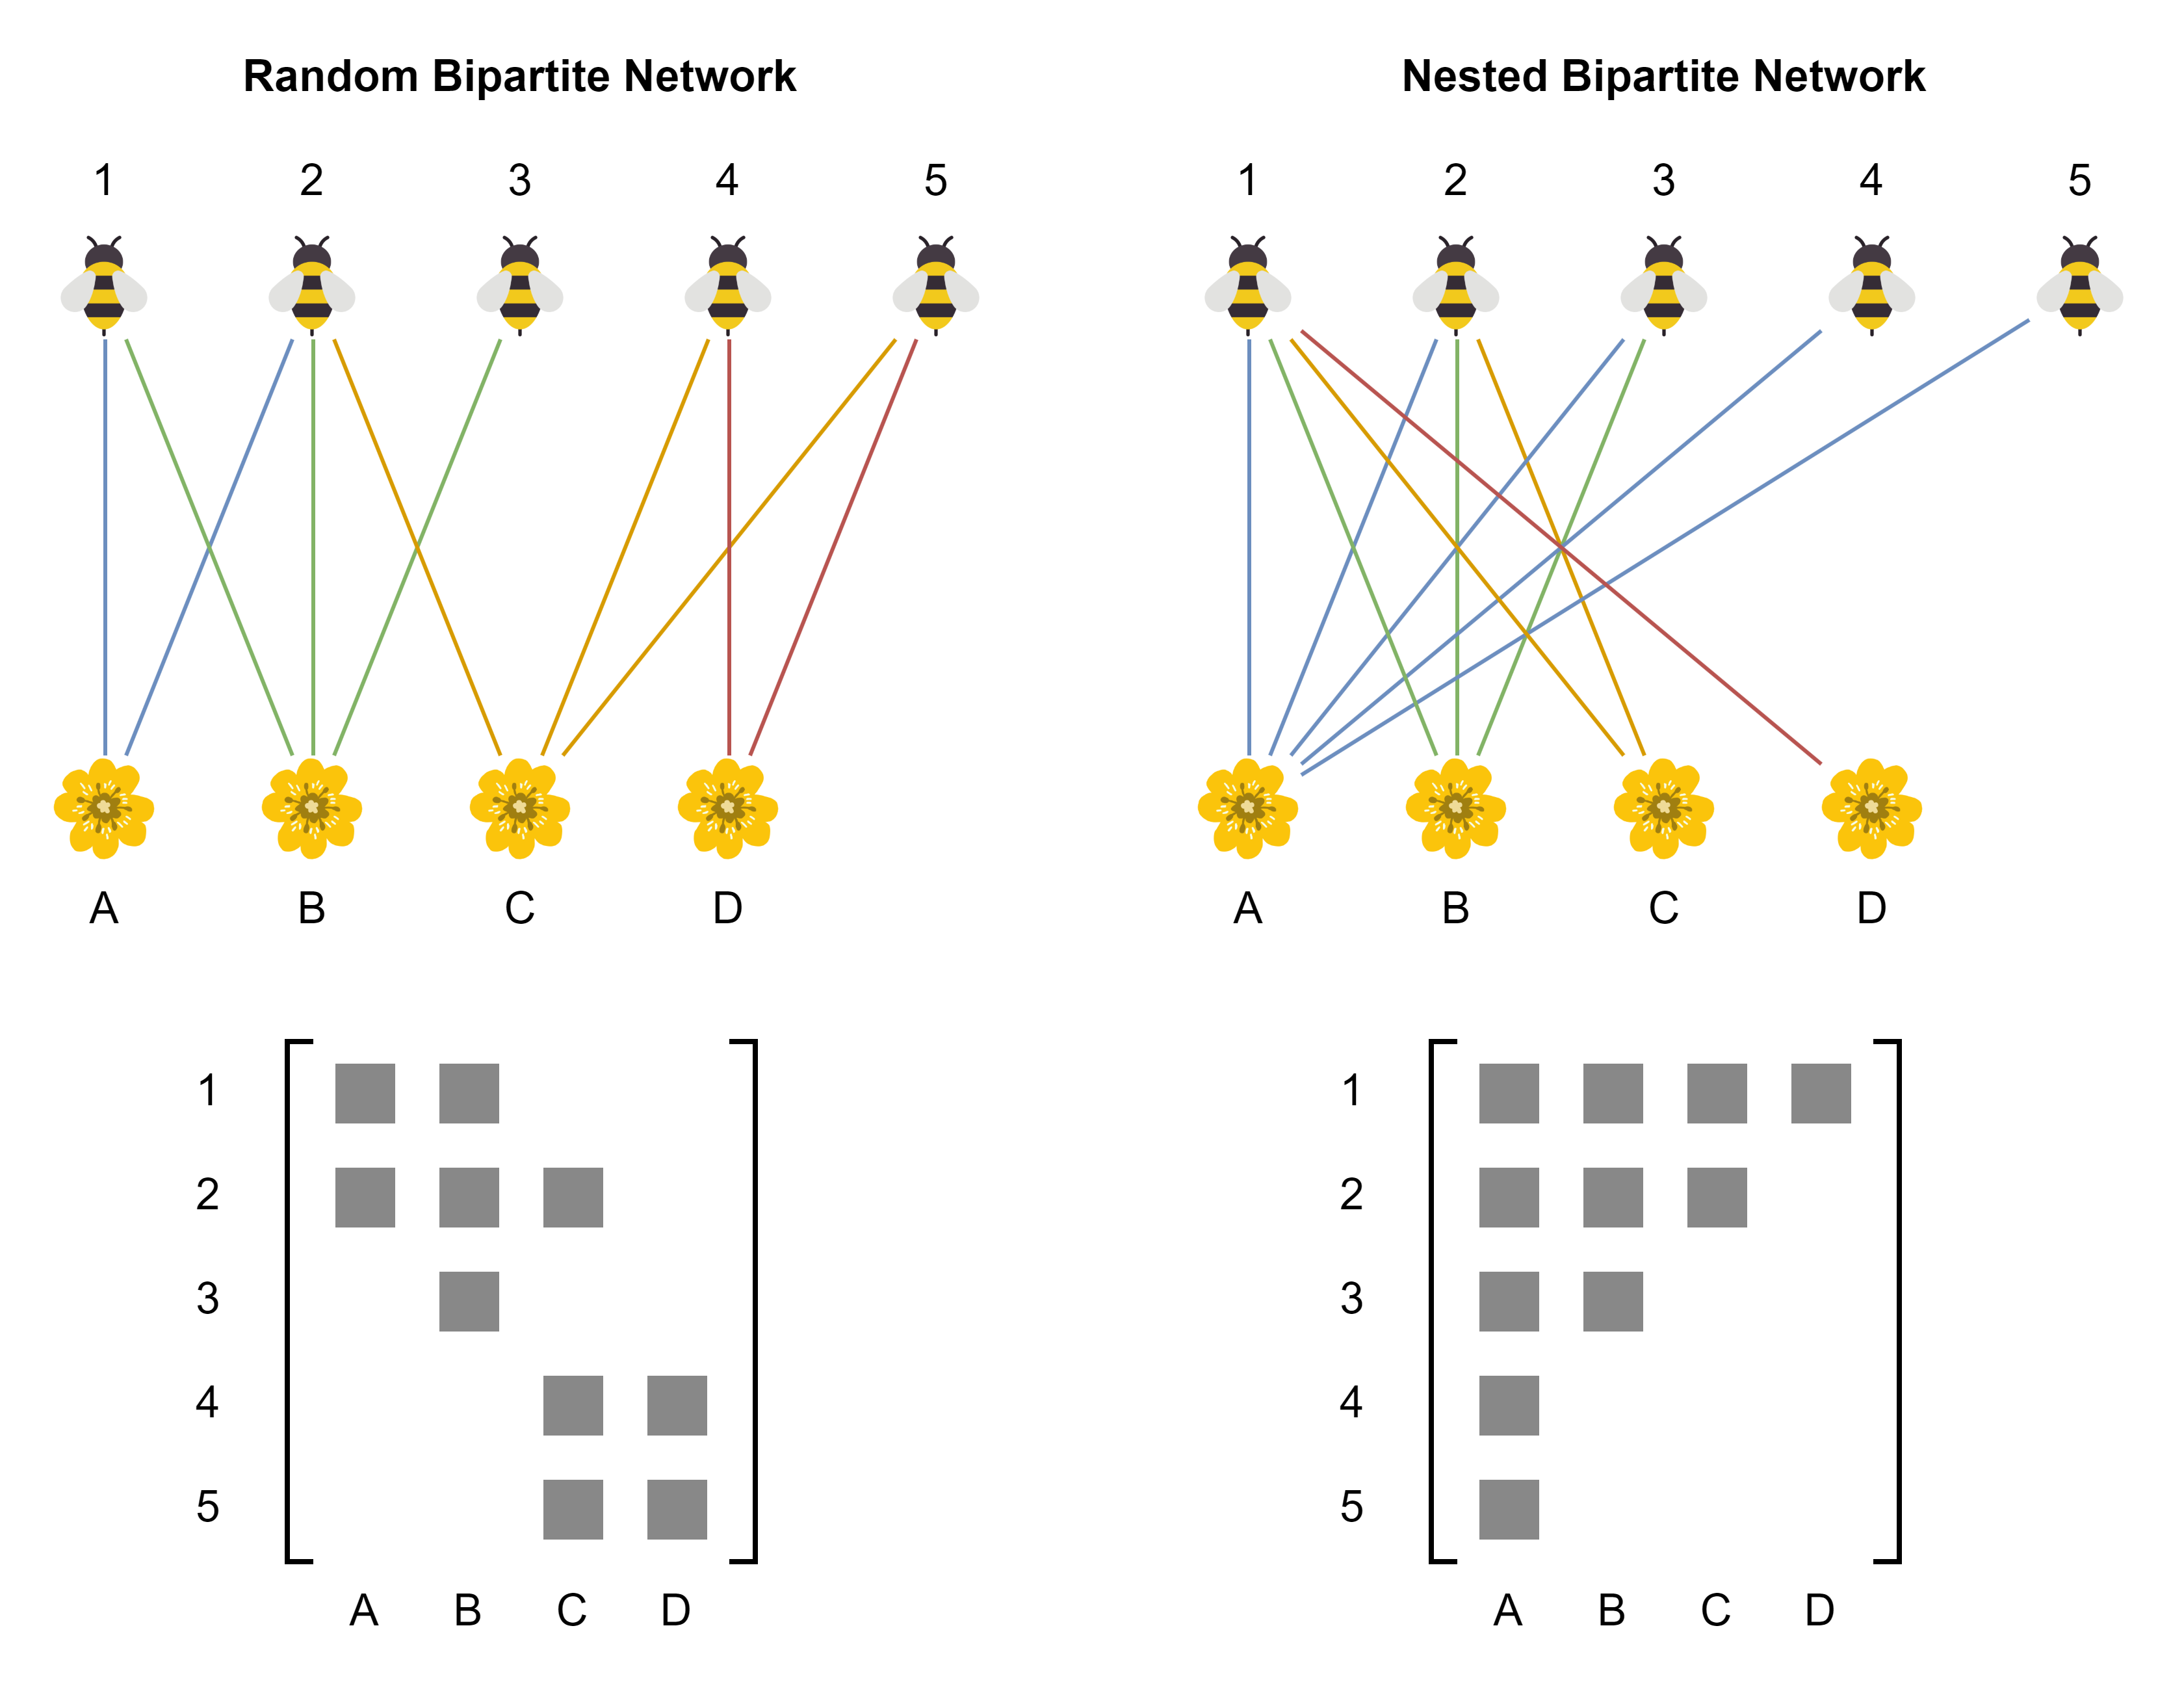
\includegraphics[width=0.7\textwidth]{../figures/diagrams/unipartite_bipartite_nested_net_v2.png}
    \caption{Nestedness in pollinator-plant networks. \textbf{Specialists} interact with subsets of the same partners as \textbf{generalists}}
\end{figure}

\end{frame}

\begin{frame}
\frametitle{Understanding Nestedness Pattern}

\begin{columns}
\begin{column}{0.5\textwidth}
\textbf{Ecological Example:}
\begin{itemize}
    \item \textcolor{blue}{Generalist pollinators} visit many plant species
    \item \textcolor{red}{Specialist pollinators} visit few plant species
    \item Specialists visit \textbf{subsets} of generalists' plants
    \item Creates triangular matrix pattern
\end{itemize}
\end{column}
\begin{column}{0.5\textwidth}
\textbf{VC Translation:}
\begin{itemize}
    \item \textcolor{blue}{Highly connected investors} have many partnerships
    \item \textcolor{red}{Less connected investors} have few partnerships
    \item Less connected investors partner with \textbf{subsets} of highly connected investors' partners
    \item Creates hierarchical organization
\end{itemize}
\end{column}
\end{columns}

\vspace{0.3cm}

\begin{alertblock}{Key Insight}
Nestedness reveals \textbf{hierarchical coordination patterns} that would be invisible in classical unipartite networks!
\end{alertblock}

\end{frame}

\begin{frame}
\frametitle{Measuring Nestedness: NODF Metric}

\textbf{NODF} = Nestedness based on Overlap and Decreasing Fill
\begin{itemize}
    \item Ranges from 0 (random) to 1 (perfect nestedness)
    \item Accounts for both connection overlap and degree differences
    \item Standard metric in ecology, novel application to finance
\end{itemize}

\vspace{0.5cm}

\begin{block}{Statistical Significance Testing}
\begin{itemize}
    \item Use \textbf{Curveball algorithm} to generate null models
    \item Preserve degree sequences while randomizing connections
    \item Test: Is observed nestedness higher than random expectation?
    \item p < 0.05 = significantly nested structure
\end{itemize}
\end{block}

\end{frame}

\begin{frame}
\frametitle{Why Nestedness Matters for Innovation}

\textbf{Implications for VCs:}
\begin{itemize}
    \item Information flow from generalists to specialists
    \item Hierarchical access to opportunities
    \item Efficiency vs. accessibility trade-offs
\end{itemize}

\vspace{0.3cm}

\textbf{Implications for Startups:}
\begin{itemize}
    \item Network position affects funding access
    \item "Gatekeeper" investors control broader networks
    \item Geographic clustering effects
\end{itemize}

\begin{alertblock}{Research Questions}
Do VC networks exhibit nestedness? How does geography influence it? When does it emerge over time?
\end{alertblock}

\end{frame}
